\clearpage
\chapter{Converting $\epsilon$-NFA to NFA}

\section{Aim}
To design and implement a program that accepts a Epsilon Non-deterministic Finite Automaton ($\epsilon$-NFA) and computes NFA without $\epsilon$ transitions.

\section{Algorithm}

\begin{algorithm}[H]
	\caption{An algorithm to convert $\epsilon$-NFA to NFA }
	\begin{algorithmic}
		\Procedure{computeTransition}{$state, symb$}
			\State \Comment{state : starting state}
			\State \Comment{inputs : input symbol}
			
			\State $resultSet \gets \{\}$ \Comment{Empty set}
			
			\State $Eset \gets \Call{EClosure}{state}$ \Comment{Computing e-closure}
			
			
			\ForAll{$Estate \in Eset$}
				\State $Tstates \gets \Call{transition}{Estate,sym}$ \Comment{set of states after transition}
				\ForAll{$subState \in Tstates$}
					\State $resultSet \gets resultSet \cup \Call{EClosure}{subState}$ \Comment{Union of eclosures}
				\EndFor
			\EndFor
			\State return $resultSet$
		\EndProcedure

		\ForAll{$state \in TotalStates$}
			\State $symbols \gets \Call{getInputSymbols}{state}$ \Comment{set of possible input symbols}
			\ForAll{$sym \in symbols$}
				\State $Eset \gets \Call{EClosure}{state}$
				\State $resultSet \gets \Call{computeTransition}{state, sym}$
				\State $\Call{print}{Eset, sym, resultSet}$
			\EndFor
		\EndFor
	\end{algorithmic}
\end{algorithm}

\subsubsection*{$\epsilon$-NFA to NFA}

\begin{figure}[H]
	\centering
	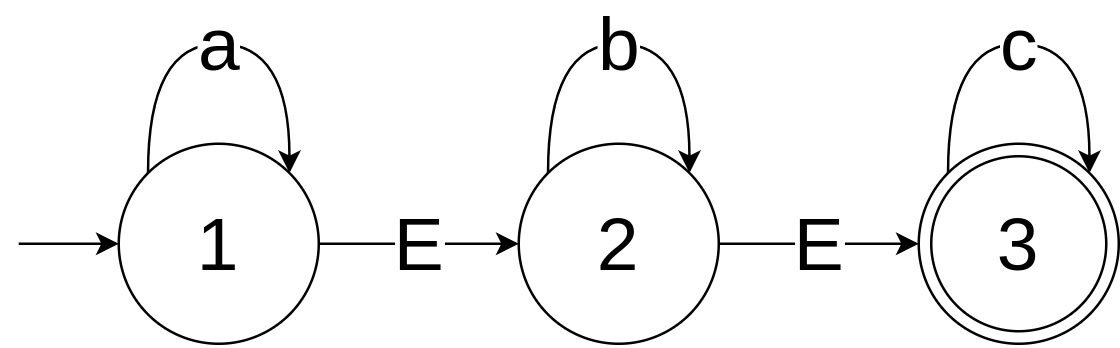
\includegraphics[width=2in]{../EXP5/diagram-ques.png}
	\caption{$\epsilon$-NFA}
\end{figure}

\begin{figure}[H]
	\centering
	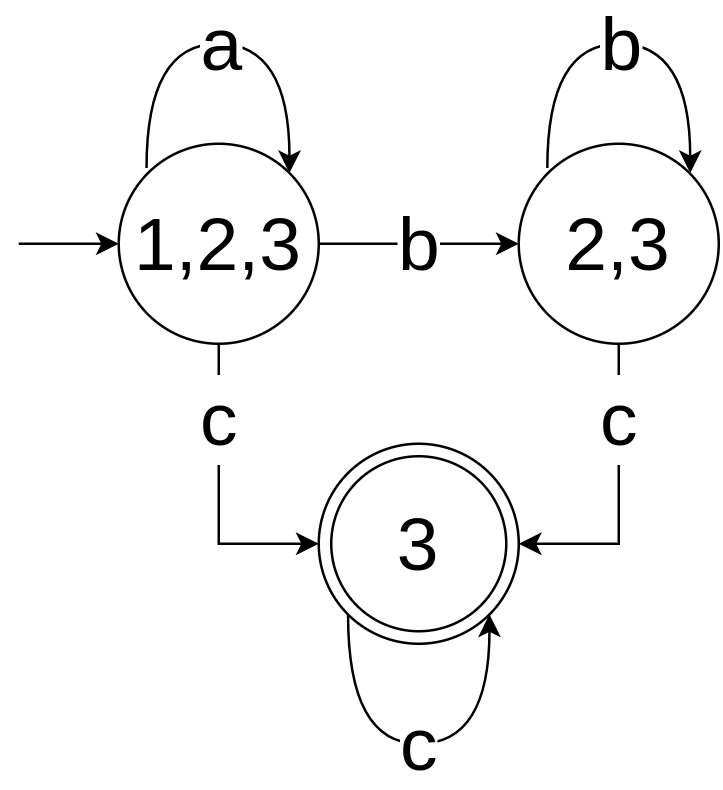
\includegraphics[height=2in]{../EXP5/diagram-ans.png}
	\caption{New NFA}
\end{figure}

\section{Python-Program}
\lstinputlisting[style=CStyle,language=python]{../EXP5/E-NFA_to_NFA.py}

\section{Output}
\lstinputlisting[style=plain]{../EXP5/output.txt}

\section{Result}
The program compiled successfully and converted $\epsilon$-NFA to NFA.